\documentclass{../c-lecture}

\subtitle{Calculation}

\begin{document}

\begin{frame}
  \titlepage{}
\end{frame}
\begin{frame}
  \frametitle{Outline}
  \tableofcontents{}
\end{frame}

\section{Produce output}

\begin{frame}[fragile]
  \frametitle{Printing}
  \begin{itemize}
    \item Printing messages
    \begin{itemize}
      \item \mint{c}|printf("This is message \n");|
    \end{itemize}
    \item Printing variables
    \begin{itemize}
      \item \mint{c}|printf("format", parameters);|
    \end{itemize}
  \end{itemize}
  \begin{minted}[bgcolor=Black]{c}
int i = 20;
char c = 'a';
printf("%d, %c", i, c);
printf("i is %d and char is %c", i, '6');
  \end{minted}
\end{frame}

\begin{frame}[fragile]
  \frametitle{Printing Integers}
  \begin{itemize}
    \item \mint{c}|%d, %i, %ld|
  \end{itemize}
  \begin{minted}[bgcolor=Black]{c}
printf("%d", 100);
// 100
printf("%d, %d", +1000, -100);
// 1000, -100
printf("%i", 100);
// 100
printf("%ld, %i", +1000, -100);
// 1000, -100
  \end{minted}
\end{frame}

\begin{frame}[fragile]
  \frametitle{Printing Unsigned Integers}
  \begin{itemize}
    \item \mint{c}|%u (base 10), %o (base 8), %x (base 16) and %X (base 16)|
  \end{itemize}
  \begin{minted}[bgcolor=Black]{c}
unsigned int i = 26;
printf("%u\n", i); // 26
printf("%o\n", i); // 32
printf("%x\n", i); // 1a
printf("%X\n", i); // 1A
  \end{minted}
\end{frame}

\begin{frame}[fragile]
  \frametitle{Printing Floats}
  \begin{itemize}
    \item \mint{c}|%f, %e, %E, %lf|
  \end{itemize}
  \begin{minted}[bgcolor=Black]{c}
printf("%f", 100.5f);
100.500000

float f = -2;
double d = 100;
printf("%f, %f", f, d);
// -2.000000, 100.000000
printf("%f, %e", 1e3, 1e3);
// 1000.000000, 1.000000e+003
  \end{minted}
\end{frame}

\begin{frame}[fragile]
  \frametitle{Printing Chars}
  \begin{itemize}
    \item \mint{c}|%c|
  \end{itemize}
  \begin{minted}[bgcolor=Black]{c}
printf("%c", 'a');
// a

printf("%c, %c", 'a','b');
// a, b

char c1 = 'a';
printf("%c, %c, %c", c1, 'b', 65);
// a, b, A
  \end{minted}
\end{frame}

\begin{frame}
  \frametitle{Special Character}
  \begin{table}
  \begin{tabular}{cc}
    \toprule

    Characters in \textit{\color{Orange} printf} &
    result \\

    \midrule

    \\n &
    newline \\

    \midrule

    \\r &
    carriage return \\

    \midrule

    \\b &
    backspace \\

    \midrule

    \\'' &
    '' \\

    \midrule

    \%\% &
    \% \\

    \midrule

    \\\%
    \%
  \end{tabular}
  \end{table}
\end{frame}

\begin{frame}[fragile]
  \frametitle{Printing Strings}
  \begin{itemize}
    \item \mint{c}|%s|
  \end{itemize}
  \begin{minted}[bgcolor=Black]{c}
printf("This is message");
// This is message

printf("This is %s", "message");
// This is message

char str1[20] = "This is message";
printf("%s", str1);
// This is message
  \end{minted}
\end{frame}

\begin{frame}
  \frametitle{Field length}
  \begin{itemize}
    \item Field length is a \textbf{\color{Orange} number}
    \item Comes after \% (and before the type char)
    \item
      It is the \textbf{\color{Green} minimum} space reserved for print

    \begin{itemize}
      \item If value is smaller than the space
      \begin{itemize}
        \item Empty space
      \end{itemize}
      \item If value is larger than the space
      \begin{itemize}
        \item No effect
      \end{itemize}
    \end{itemize}
  \end{itemize}
\end{frame}

\begin{frame}[fragile]
  \frametitle{Field length}
  \begin{minted}[bgcolor=Black]{c}
printf("|%4d|\n", 1);       // |    1|
printf("|%4d|\n", 12345);   // |12345|
printf("|%4d|\n", -12345);  // |-12345|
printf("|%4f|\n", 1234.0);  // |1234.000000|
printf("|%15f|\n", 1234.0); // |    1234.000000|
printf("|%4c|\n", 'A');     // |   A|
printf("|%4s|\n", "ABC");   // | ABC|
printf("|%4s|\n", "ABCDE"); // |ABCDE|
  \end{minted}
\end{frame}

\begin{frame}
  \frametitle{Precision}
  \begin{itemize}
    \item Precision is a \textit{\color{LimeGreen} .number} and comes after \%

    \item For Integer
    \begin{itemize}
      \item The \textit{\color{LimeGreen} minimum} number of digits
      \item If (\# of digits < precision) then empty space filled with 0
    \end{itemize}

    \item For floats
    \begin{itemize}
      \item With \%f, \%e
      \item The number of digits \textbf{\color{Cyan} after .}
    \end{itemize}

    \item For strings
    \begin{itemize}
      \item The \textbf{\color{Orange} maximum} number of characters
    \end{itemize}
  \end{itemize}
\end{frame}

\begin{frame}[fragile]
  \frametitle{Precision}
  \begin{minted}[bgcolor=Black]{c}
printf("|%.4d|\n", 1); // |0001|
printf("|%.4d|\n", 12345); // |12345|
printf("|%.4d|\n", -12345); // |-12345|
printf("|%.4f|\n", 1234.0); // |1234.0000|
printf("|%.10f|\n", 1234.0);// |1234.0000000000|
printf("|%.4s|\n", "ABC"); // |ABC|
printf("|%.4s|\n", "ABCDEF"); // |ABCD|
  \end{minted}
\end{frame}

\begin{frame}
  \frametitle{Field length and Precision}
  \begin{itemize}
    \item This is a number with format \textit{\color{Cyan} a.b}
    \item First \textit{\color{Orange} b} determines the precision
    \item Then \textit{\color{LimeGreen} a} specifies the field length
  \end{itemize}
\end{frame}

\begin{frame}[fragile]
  \frametitle{Field length and Precision}
  \begin{minted}[bgcolor=Black]{c}
printf("|%10.5d|\n", 12);
// | 00012|

printf("|%3.5d|\n", 12);
// |00012|

printf("|%10.5f|\n", 1.234567890123);
// | 1.23457|

printf("|%0.5f|\n", 1.234567890123);
// |1.23457|

printf("|%15.10s|\n", "Hello, world");
// | Hello, wor|

printf("|%5.10s|\n", "Hello, world");
// |Hello, wor|
  \end{minted}
\end{frame}

\begin{frame}[fragile]
  \frametitle{Variable Field Length \& Precision : *}
  \begin{itemize}
    \item
      * can be used to specify field length and precision which is replaced by a
      variable

  \end{itemize}
  \begin{minted}[bgcolor=Black]{c}
int i = 30;
int j = 2;
float f = 1.23456789;
printf("%0*.*f\n", i, j, f);

// 000000000000000000000000001.23
  \end{minted}
\end{frame}

\begin{frame}[fragile]
  \frametitle{Cast in printing (do NOT use)}
  \begin{minted}[bgcolor=Black]{c}
int i = -60;
unsigned int j = 4147482648;
float f = -700.05;

printf("i = %f\n", i);
// i = 0.000000

printf("i = %u\n", i);
// i = 4294967236

printf("j = %d\n", j);
// j = -147484648

printf("f = %d\n", f);
// f = 1610612736
  \end{minted}
\end{frame}

\section{Get input values}

\begin{frame}[fragile]
  \frametitle{Reading}
  \begin{itemize}
    \item Read from keyboard (console)
    \item What should be determined in reading
    \begin{itemize}
      \item Keyboard enters ``characters'', so, how to read int, char, …?
      \item Which type the chars should be converted?
      \item Where should be saved?
    \end{itemize}
    \item \mint{c}|scanf("format", parameters)|
    \begin{itemize}
      \item Format: The type that input should be converted to
      \item Parameters: Where should be saved
    \end{itemize}
    \item scanf blocks until ‘Enter’ at the end of input (why?!)
    \item Reads from beginning until to white spaces (except reading chars)
  \end{itemize}
\end{frame}

\begin{frame}[fragile]
  \frametitle{Reading Integers (base 10)}
  \begin{itemize}
    \item \mint{c}|%d, %u, %ld, %lu|
  \end{itemize}
  \begin{minted}[bgcolor=Black]{c}
int i;
unsigned int j;
long int l;
scanf("%d", &i); // -90
scanf("%u", &j); // 78
scanf("%ld", &l); // 60

// -90 is saved in memory location i
// 78 is saved in memory location j
// 60 is saved in memory location l

  \end{minted}
  \begin{block}{}
  Spaces at the beginning are ignored
  \end{block}
\end{frame}

\begin{frame}[fragile]
  \frametitle{Reading Integers (cont’d)}
  \begin{itemize}
    \item \mint{c}|%o, %x, %X, %i|
  \end{itemize}
  \begin{minted}[bgcolor=Black]{c}
scanf("%o", &i);
// Input: 12 → i = 10

scanf("%x", &i);
// Input: 1a → i = 26

scanf("%i", &i);
// Input: 12 → i = 12
// Input: 012 → i = 10 (It reads in base 8)
// Input: 0x12 → i = 18 (It reads in base 16)
  \end{minted}
\end{frame}

\begin{frame}[fragile]
  \frametitle{Reading floats and doubles}
  \begin{itemize}
    \item \mint{c}|%f, %lf, %e|
  \end{itemize}
  \begin{minted}[bgcolor=Black]{c}
float f;
double d;
scanf("%f", &f);
scanf("%lf", &d);

// 90.9 → 90.9 is saved in memory f
// 88.123456789 → 88.123456789 saved in memory d
  \end{minted}
  \begin{block}{}
  Spaces at the beginning are ignored
  \end{block}
\end{frame}

\begin{frame}[fragile]
  \frametitle{Reading floats and doubles}
  \begin{minted}[bgcolor=Black]{c}
float f1, f2;
scanf("%f", &f1);
scanf("%e", &f2);

// 1.23 → f1 = 1.23
// 4.56 → f2 = 4.56

// 1.23e+1 → f1 = 12.3
// 4.56e-1 → f2 = 0.456
  \end{minted}
\end{frame}

\begin{frame}[fragile]
  \frametitle{Reading chars}
  \begin{itemize}
    \item \mint{c}|%c|
  \end{itemize}
  \begin{minted}[bgcolor=Black]{c}
char c1, c2, c3;
scanf("%c", &c1); /* spaces */
scanf("%c", &c2);
scanf("%c", &c3);

// azb →
// c1 = 'a'
// c2 = 'z'
// c3 = 'b'
  \end{minted}
  \begin{block}{}
  Spaces at the beginning are NOT ignored
  \end{block}
\end{frame}

\begin{frame}[fragile]
  \frametitle{Reading chars (cont’d)}
  \begin{itemize}
    \item White spaces (space, tab, enter) are not ignored when reading char
    \item To ignore white spaces, use '' `` before \%c
  \end{itemize}
  \begin{minted}[bgcolor=Black]{c}
scanf("%d%c%d", &i, &c, &j);
Input: 123 45 → I = 123 c = ‘ ‘ j = 45

scanf("%d %c%d", &i, &c, &j);
Input: 123 4 56 → I = 123 c = ‘4’ j = 56
Input: 123 456 → I = 123 c = ‘4’ j = 56
  \end{minted}
\end{frame}

\begin{frame}
  \frametitle{Reading chars (cont’d)}
  \begin{itemize}
    \item getchar()
    \begin{itemize}
      \item Read char <span class="hl-orange">after Enter</span>
    \end{itemize}
    \item getch()
    \begin{itemize}
      \item
        Read char <span class="hl-orange">without Enter</span>,
        <span class="hl-green">does NOT show</span> the char

    \end{itemize}
    \item getche()
    \begin{itemize}
      \item
        Read char <span class="hl-orange">without Enter</span>,
        <span class="hl-green">shows</span> the char

    \end{itemize}
  \end{itemize}
\end{frame}

\begin{frame}[fragile]
  \frametitle{Reading Strings}
  \begin{itemize}
    \item How to read a line
    \item Contains spaces (read until end of line)
    \item gets(s)
  \end{itemize}
  \begin{minted}[bgcolor=Black]{c}
char str[20];
gets(str);

Input: ABC DEF → str = "ABC DEF"
  \end{minted}
\end{frame}

\begin{frame}[fragile]
  \frametitle{Field length in scanf}
  \begin{itemize}
    \item
      Field length specifies the <span class="hl-orange">maximum</span> number
      of input characters (in the buffer) used for scanning

  \end{itemize}
  \begin{minted}[bgcolor=Black]{c}
int i, j;

scanf("%5d", &i);
Input: 122 → i = 122
Input: 1234567 → i = 12345

scanf("%5d%d", &i, &j);
Input: 1 2 → i = 1, j = 2
Input: 1234567 → i = 12345, j = 67
Input: 123456 7 → i = 12345, j = 6
  \end{minted}
\end{frame}

\begin{frame}[fragile]
  \frametitle{Special input format}
  \begin{itemize}
    \item If input data has special format with extra characters
    \item scanf can ignore them
  \end{itemize}
  \begin{minted}[bgcolor=Black]{c}
int y, m, d;
scanf("%d/%d/%d", &y, &m, &d);

Input: 1389/12/1 → y = 1389, m = 12, d = 1
  \end{minted}
\end{frame}

\begin{frame}[fragile]
  \frametitle{Format of actual input data}
  \begin{itemize}
    \item
      The format of actual input data <span class="hl-orange">MUST</span> match
      with the format of scanf

  \end{itemize}
  \begin{minted}[bgcolor=Black]{c}
int a, b;
float f;
scanf("%d--%d%f", &a, &b, &f);

Input: 1--2 3.0 → a = 1, b = 2, f = 3.0
Input: 1-2 3.0 → a = 1, b = 57, f = 0.0
Input: 1.0--2 3.0 → a = 1, b = 57, f = 0.0
  \end{minted}
\end{frame}

\begin{frame}[fragile]
  \frametitle{Common Bugs}
  \begin{itemize}
    \item Casting in printf or scanf
    \begin{itemize}
      \item \mint{c}|printf("%d", 120.23);|
      \item \mint{c}|double d; scanf("%f", &d);|
    \end{itemize}
    \item Mismatch between format and the number of expressions
    \begin{itemize}
      \item \mint{c}|printf("%d %d", 10);|
      \item \mint{c}|printf("%d", 10, 20);|
    \end{itemize}
    \item
      Using name of variable instead of \textbf{\color{Orange} address}
    \begin{itemize}
      \item \mint{c}|scanf("%d", i);|
    \end{itemize}
  \end{itemize}
\end{frame}

\begin{frame}
  \frametitle{Legends}
  \begin{figure}
    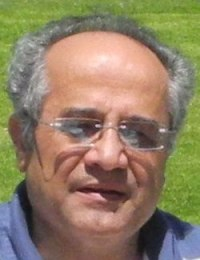
\includegraphics[height=.75\textheight]{./img/ghodsi.jpg}
  \end{figure}
  \pause%
  \centering
  \color{Violet} Mohammad Ghodsi
\end{frame}

\end{document}
